\section{\IT{И} и \IT{ИЛИ} как вычитание и сложение}

\subsection{Текстовые строки в \ac{ROM} ZX Spectrum}
\label{ZX Spectrum}

Те, кто пытался исследовать внутренности \ac{ROM} ZX Spectrum-а, вероятно, замечали,
что последний символ каждой текстовой строки как будто бы отсутствует.

\begin{figure}[H]
\centering
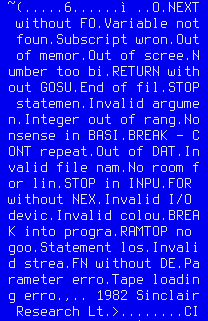
\includegraphics[width=0.3\textwidth]{fundamentals/zx_spectrum_ROM.png}
\caption{Часть \ac{ROM} ZX Spectrum}
\end{figure}

На самом деле, они присутствуют.

Вот фрагмент из дизассемблированного \ac{ROM} ZX Spectrum 128K:

\lstinputlisting{fundamentals/ZX_Spectrum_ROM.lst}
( \url{http://www.matthew-wilson.net/spectrum/rom/128_ROM0.html} )

Последний символ имеет выставленный старший бит, который означает конец строки.
Вероятно, так было сделано, чтобы сэкономить место?
В старых 8-битных компьютерах был сильный дефицит памяти.

Символы всех сообщений всегда находятся в стандартной 7-битной \ac{ASCII}-таблице, так что это гарантия,
что 8-й бит никогда не используется для символов.

Чтобы вывести такую строку, мы должны проверять \ac{MSB} каждого байта, и если он выставлен, мы должны его сбросить,
затем вывести символ, затем остановиться.
Вот пример на Си:

\begin{lstlisting}[style=customc]
unsigned char hw[]=
{
	'H',
	'e',
	'l',
	'l',
	'o'|0x80
};

void print_string()
{
	for (int i=0; ;i++)
	{
		if (hw[i]&0x80) // проверить MSB
		{
			// сбросить MSB
			// §(иными словами, сбросить всё, но оставить нетронутыми младшие 7 бит)§
			printf ("%c", hw[i] & 0x7F);
			// остановиться
			break;
		};
		printf ("%c", hw[i]);
	};
};
\end{lstlisting}

И вот что интересно, так как 8-й бит это самый старший бит (в байте), мы можем проверить его, выставить и сбросить
используя арифметические операции вместо логических.

Я могу переписать свой пример на Си:

\begin{lstlisting}[style=customc]
unsigned char hw[]=
{
	'H',
	'e',
	'l',
	'l',
	'o'+0x80
};

void print()
{
	for (int i=0; ;i++)
	{
		// hw[] должен иметь тип 'unsigned char'
		if (hw[i] >= 0x80) // проверить MSB
		{
			printf ("%c", hw[i]-0x80); // сбросить MSB
			// останов
			break;
		};
		printf ("%c", hw[i]);
	};
};
\end{lstlisting}

\IT{char} по умолчанию это знаковый тип в \CCpp, так что, чтобы сравнивать его с переменной вроде 0x80 (которая отрицательная
($-128$),
если считается за знаковую),
мы должны считать каждый символ сообщения как беззнаковый.

Теперь, если 8-й бит выставлен, число всегда больше или равно 0x80.
Если 8-й бит сброшен, число всегда меньше 0x80.

И даже более того: если 8-й бит выставлен, его можно сбросить вычитанием 0x80, и ничего больше.
Если он уже сброшен, впрочем, операция вычитания уничтожит другие биты.

Точно также, если 8-й бит сброшен, можно его выставить прибавлением 0x80.
Но если он уже выставлен, операция сложения уничтожит остальные биты.

На самом деле, это справедливо для любого бита.
Если 4-й бит сброшен, вы можете выставить его просто прибавлением 0x10: 0x100+0x10 = 0x110.
Если 4-й бит выставлен, вы можете его сбросить вычитанием 0x10: 0x1234-0x10 = 0x1224.

Это работает, потому что перенос не случается во время сложения/вычитания.
Хотя, он случится если бит уже выставлен перед сложением или сброшен перед вычитанием.

Точно также, сложение/вычитание можно заменить на операции \IT{ИЛИ/И} если справедливы два условия:
1) вы хотите прибавить/вычесть число вида $2^n$;
2) бит в исходном значение сброшен/выставлен.

Например, прибавление 0x20 это то же что и применение \IT{ИЛИ} со значением 0x20 с условием что этот бит был сброшен перед
этим:
0x1204|0x20 = 0x1204+0x20 = 0x1224.

Вычитание 0x20 это то же что и применение \IT{И} со значением ~0x20 (0x....FFDF), но если этот бит был выставлен до этого:
0x1234\&(\~{}0x20) = 0x1234\&0xFFDF = 0x1234-0x20 = 0x1214.

Опять же, это работает потому что перенос не случается если вы прибавляете число вида $2^n$ и этот бит до этого сброшен.

Это важное свойство булевой алгербы, его стоит понимать и помнить о нем.

